% Full paperback cover (back, spine, front) of the TypeScript edition for KDP.
% Build it with make-cover.sh, which also converts ../back-cover.txt into back-text.tex.
\documentclass{article}
\usepackage[T1]{fontenc}
\usepackage{mathpazo}
\usepackage{microtype}
\usepackage{graphicx}
\usepackage{xcolor}
\usepackage{tikz}
\usepackage{enumitem}
\usepackage{url}
\urlstyle{same}

% Book data: KDP's spine width is the page count times the paper thickness
% (premium color: 0.002347 in per page).
\newcommand{\pages}{188}
\newcommand{\perpage}{0.002347in}
\newif\ifguides
\ifdefined\withguides\guidestrue\fi  % trim lines, fold lines, safe zones, barcode area

\newlength{\bleed}  \setlength{\bleed}{0.125in}
\newlength{\trimW}  \setlength{\trimW}{8.5in}
\newlength{\trimH}  \setlength{\trimH}{11in}
\newlength{\spine}  \setlength{\spine}{\dimexpr \perpage * \pages \relax}
\newlength{\coverW} \setlength{\coverW}{\dimexpr 2\bleed + 2\trimW + \spine \relax}
\newlength{\coverH} \setlength{\coverH}{\dimexpr 2\bleed + \trimH \relax}
\newlength{\spineL} \setlength{\spineL}{\dimexpr \bleed + \trimW \relax}  % left fold
\newlength{\spineR} \setlength{\spineR}{\dimexpr \spineL + \spine \relax} % right fold

\setlength{\paperwidth}{\coverW}  \setlength{\pdfpagewidth}{\coverW}
\setlength{\paperheight}{\coverH} \setlength{\pdfpageheight}{\coverH}
\setlength{\hoffset}{-1in}  \setlength{\voffset}{-1in}
\setlength{\oddsidemargin}{0pt} \setlength{\topmargin}{0pt}
\setlength{\headheight}{0pt} \setlength{\headsep}{0pt}
\setlength{\textwidth}{\coverW} \setlength{\textheight}{\coverH}
\setlength{\parindent}{0pt}
\pagestyle{empty}

\definecolor{ink}{RGB}{58,38,28}     % dark brown of the title on the front
\definecolor{slate}{RGB}{84,98,122}  % blue gray of the ornaments in the frame

\begin{document}
\begin{tikzpicture}[inner sep=0pt, outer sep=0pt]
  \useasboundingbox (0,0) rectangle (\coverW,\coverH);
  % backgrounds: parchment for back and spine, the illustration for the front
  \node[anchor=south west] at (0,0)
       {
\includegraphics[width=\spineR, height=\coverH]{parchment-back.jpg}};
  \node[anchor=south west] at (\spineR,0)
       {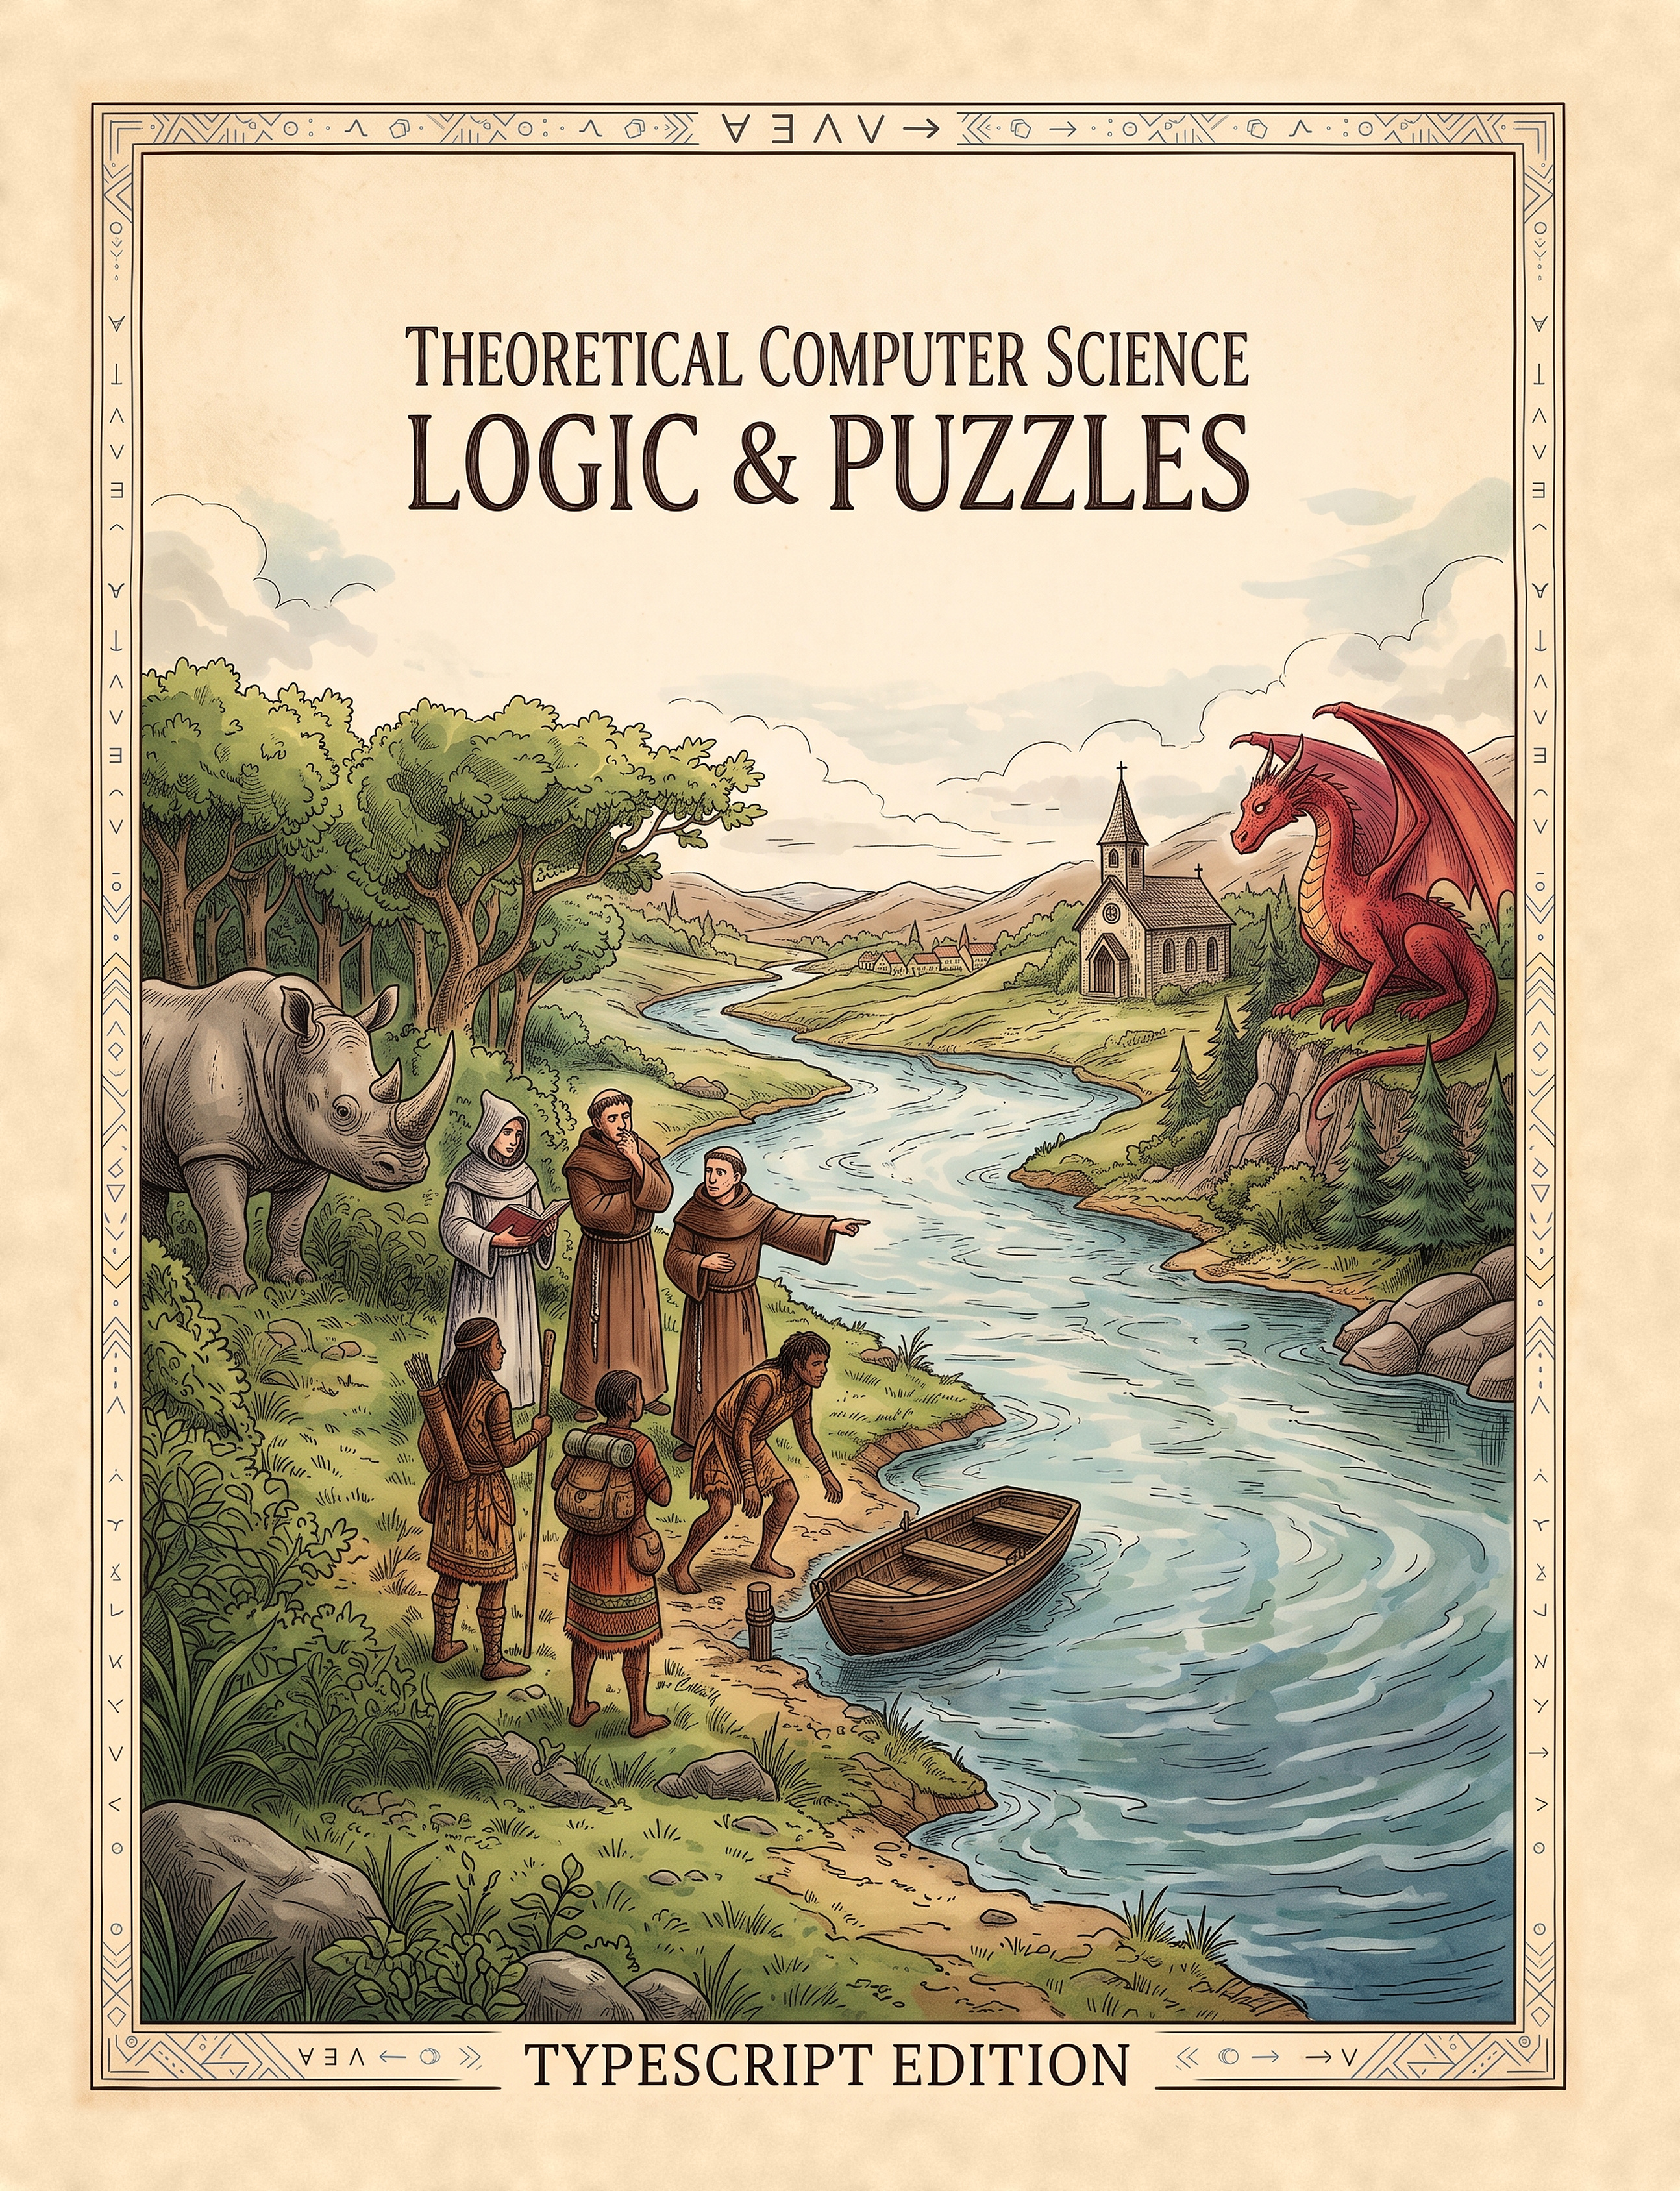
\includegraphics[width=\dimexpr\coverW-\spineR\relax, height=\coverH]{../lecture-notes-cover-print.jpg}};

  % back cover: ornament and text, kept clear of the barcode area in the lower right corner
  \node[anchor=north, text width=6.4in, color=ink, align=justify]
       at ({\bleed+0.5*\trimW}, {\coverH-\bleed-1.3in}) {%
    {\centering\color{slate}\rule[0.5ex]{1.2in}{0.6pt}\quad
     \Large$\forall\;\;\exists\;\;\wedge\;\;\vee\;\;\rightarrow$\quad
     \rule[0.5ex]{1.2in}{0.6pt}\par}
    \vspace{0.35in}
    \fontsize{13.5}{18.5}\selectfont\frenchspacing
    \setlist[itemize]{leftmargin=1.6em, itemsep=1pt, topsep=3pt,
                      label={\color{slate}\textbullet}}
    Can a program decide whether another program will ever stop? How do you prove that a function is correct for every input, not just for the ones you tested? How does a computer find a proof on its own? This book answers these questions with precise definitions, complete proofs, and working TypeScript programs.
\par\medskip

Every central idea becomes code. You implement a formula evaluator, the conversion to conjunctive normal form, the Davis-Putnam SAT solver, a backtracking constraint solver, and the unification algorithm. Then you use industrial tools, the SAT solver MiniSat, Microsoft's Z3, and the theorem provers Vampire, Prover9, and Mace4, to see how far the same ideas reach.
\par\medskip

Topics include
\begin{itemize}
\item correctness proofs by computational induction and symbolic execution
\item propositional logic, normal forms, and the Davis-Putnam algorithm
\item first-order logic and constraint programming
\item automated theorem proving with resolution and unification
\end{itemize}
\par\medskip

Along the way you place eight queens on a chessboard, solve the Zebra Puzzle and a Sudoku, lead a knight across all 64 squares, and find out who killed Aunt Agatha.
\par\medskip

Written for first-year students of computer science and for every programmer who wants to reason precisely about software. All programs are available as Jupyter notebooks at \url{github.com/karlstroetmann/Logic}.
\par\medskip

Karl Stroetmann is a professor at the Baden-Wuerttemberg Cooperative State University (DHBW), where this book grew out of a course on theoretical computer science. Until 2002 the author worked on hardware verification at the Siemens Research Center.
\par\medskip


  };

  % spine, read from top to bottom
  \node[anchor=west, rotate=-90, color=ink]
       at ({\spineL+0.5*\spine}, {\coverH-\bleed-0.6in})
       {\fontsize{12}{12}\selectfont\scshape Theoretical Computer Science\quad
        \fontsize{16}{16}\selectfont\bfseries Logic \& Puzzles\quad
        \fontsize{11}{11}\selectfont\mdseries\upshape TypeScript Edition};
  \node[anchor=east, rotate=-90, color=ink]
       at ({\spineL+0.5*\spine}, {\bleed+0.6in})
       {\fontsize{13}{13}\selectfont Karl Stroetmann};

  \ifguides
    \draw[red, very thin] (\bleed,\bleed) rectangle ({\coverW-\bleed}, {\coverH-\bleed});
    \draw[red, very thin] (\spineL,0) -- (\spineL,\coverH) (\spineR,0) -- (\spineR,\coverH);
    \draw[blue, very thin, dashed] ({2*\bleed}, {2*\bleed})
         rectangle ({\spineL-\bleed}, {\coverH-2*\bleed});
    \draw[blue, very thin, dashed] ({\spineR+\bleed}, {2*\bleed})
         rectangle ({\coverW-2*\bleed}, {\coverH-2*\bleed});
    \fill[white, opacity=0.8] ({\spineL-0.25in-2in}, {\bleed+0.25in})
         rectangle ({\spineL-0.25in}, {\bleed+1.45in});
  \fi
\end{tikzpicture}
\end{document}
